% Packages

\documentclass[12pt]{article}
\usepackage[letterpaper, margin=1in, utf8]{geometry}
\usepackage{fancyhdr, graphicx, xcolor, wrapfig, hyperref}
\usepackage[thinlines]{easytable}
\graphicspath{ {./images/} }

\newcommand{\red}[1]{\(\color{red}#1\)}

\pagestyle{fancy} % Utilisation de fancyhdr

% -------------------------

% Première page

\title{\Huge\textbf{Quack - Le Jeu d'échecs (scolaire)}}
\date{Juin 2025}

% -------------------------

\begin{document}
\maketitle

% Mise en page footer / header

\renewcommand{\headrulewidth}{0mm} % Vire la ligne du header
\renewcommand{\footrulewidth}{0.1mm} % Redimensionne la ligne du footer
\rhead{QUACK}
\lfoot{EPITA 2027}

% ------------------------------

\centerline{Groupe 2}
\vspace{\fill}
Lépine Marc-Aurèle \par
Battistella Alexis \par
Loup Thomas \par
Maston Claudia \par
Delrieu Nathan

% Nom du groupe

% /-------------------\
% | Début du Document |
% \-------------------/

\newpage

\renewcommand\contentsname{\centering Table des matières}
% Remplace le nom par défaut de la Table des matières
\renewcommand\footnoterule{}
% Supprime la ligne séparatrice des footnotes

\tableofcontents
% Créé une table des matières à partir des sections, subsections et subsubsections

\newpage

\section{Introduction}
Le \href{https://www.youtube.com/watch?v=LFwXghcajLw&list=PLtn704u3JW-K4q9YkQWTfWRxaq-9oLfJ3&index=4}{jeu d'échecs à quatre cases} est une énigme quantique dont le but est de faire deviner l'emplacement d'une clé. Cette dernière est cachée sous l'une des cases de l'échiquier.\newline
\newline
La composition de l'échiquier est simple : sur chaque case, on retrouve une pièce qui indique soit la valeur 0 (pile) soit la valeur 1 (face).\newline
\newline
Voici comment se déroule une partie dans la configuration 2x2 :
\newline
- Un premier joueur découvre la grille et connaît la position de la clé. Il n'a le droit de retourner qu'une seule pièce afin de faire deviner la position de la clé au second joueur.
\newline
- Le second joueur découvre ensuite la grille et doit trouver l'emplacement de la clé grâce aux valeurs des pièces.\newline
\newline
Ce problème, travaillant sur les notions de superposition, de parité et de contrôle par l'état 0, ne présente pas d'avantage quantique en raison de sa solution simple.\newline
\newline
Explication de la stratégie :\newline
Tout d'abord, on découpe la grille 2x2 en attribuant des indices binaires à chacune des cases: le premier indice indique la ligne et le deuxième la colonne (cf. 2.1).\newline
Les deux joueurs vont ensuite, avant le début du jeu, se mettre d'accord sur une case où se concentrer (admettons ici la case d'indices 11). Nous nous servons alors de la somme en binaire des valeurs des pièces sur la ligne d'indice 1 pour indexer la ligne de la clé et de la somme en binaire des valeurs des pièces sur la colonne d'indice 1 pour indexer la colonne de la clé.\newline
Ainsi, en suivant cette stratégie, le premier joueur peut toujours indiquer la réponse en suivant ces règles :\newline
- Si seule la $\Sigma$ mod 2 sur la ligne est $\ne$ de la ligne de la clé, alors il devra tourner la pièce 10.\newline
- Si seule la $\Sigma$ mod 2 sur la colonne est $\ne$ de la colonne de la clé, alors il devra tourner la pièce 01.\newline
- Si les deux sommes n'indiquent pas le bon emplacement, alors il tournera la pièce 11.\newline
- Enfin, si les sommes indiquent déjà le bon emplacement, alors il tournera la pièce 00.\newline
\newline
Dans le cadre de ce projet, nous allons nous intéresser à développer deux algorithmes pour résoudre deux variantes de cette énigme : le jeu d'échecs 4x4 et le jeu d'échecs 8x8.
  
\section {Description}
    \subsection{Découpage de la grille}
    Nous avons choisi de découper la grille de manière récursive de telle sorte à pouvoir travailler de manière récursive sur des grilles 2x2 comme celle-ci :

    \label{sec:grid-2x2}
    \begin{center}
        \begin{TAB}(4,2cm,2cm, 2cm, 2cm)[5pt]{|c|c|}{|c|c|}% (rows,min,max)[tabcolsep]{columns {rows}
            00 & 01 \\
            10 & 11 \\
        \end{TAB}
    \end{center}

    \subsubsection{Grille 4x4}
    Dans cette variante, nous pouvons tourner 2 pièces.
    \begin{center}
        \begin{TAB}(4,2cm,2cm, 2cm, 2cm)[5pt]{|c|c|c|c|}{|c|c|c|c|}% (rows,min,max)[tabcolsep]{columns}{rows}
        \textcolor{red}{00}00 & \textcolor{red}{00}01 & \textcolor{red}{01}00 & \textcolor{red}{01}01 \\
        \textcolor{red}{00}10 & \textcolor{red}{00}11 & \textcolor{red}{01}10 & \textcolor{red}{01}11 \\
        \textcolor{red}{10}00 & \textcolor{red}{10}01 & \textcolor{red}{11}00 & \textcolor{red}{11}01 \\
        \textcolor{red}{10}10 & \textcolor{red}{10}11 & \textcolor{red}{11}10 & \textcolor{red}{11}11 \\
        \end{TAB}
    \end{center}

    Les deux Qbits en \textcolor{red}{rouge} donnent la position de la sous-grille et les deux noirs donnent la position de la clé dans la sous-grille.
    \newline
    \newline
    On va appliquer l'algorithme de résolution d'une grille 2x2 sur la grille 11 pour déterminer la sous-grille 2x2 dans laquelle est la clé, et ensuite faire de même sur la grille 00 pour déterminer l'emplacement de la clé dans la sous-grille trouvée.

    \subsubsection{Grille 8x8}


    \newpage
    Dans cette variante, nous pouvons tourner 3 pièces.
    Le principe est exactement le même pour la version 8x8 (c'est juste moins lisible ;-;).
        \begin{center}
        \begin{TAB}(4,2cm,2cm, 2cm, 2cm)[5pt]{|c|c|c|c|c|c|c|c|}{|c|c|c|c|c|c|c|c|}% (rows,min,max)[tabcolsep]{columns}{rows}
        \textcolor{red}{00}\textcolor{blue}{00}000 & \textcolor{red}{00}\textcolor{blue}{00}01 & \textcolor{red}{00}\textcolor{blue}{01}00 & \textcolor{red}{00}\textcolor{blue}{01}01 & \textcolor{red}{01}\textcolor{blue}{00}00 & \textcolor{red}{01}\textcolor{blue}{00}01 & \textcolor{red}{01}\textcolor{blue}{01}00 & \textcolor{red}{01}\textcolor{blue}{01}01 \\
        \textcolor{red}{00}\textcolor{blue}{00}10 & \textcolor{red}{00}\textcolor{blue}{00}11 & \textcolor{red}{00}\textcolor{blue}{01}10 & \textcolor{red}{00}\textcolor{blue}{01}11 & \textcolor{red}{01}\textcolor{blue}{00}10 & \textcolor{red}{01}\textcolor{blue}{00}11 & \textcolor{red}{01}\textcolor{blue}{01}10 & \textcolor{red}{01}\textcolor{blue}{01}11 \\
        \textcolor{red}{00}\textcolor{blue}{10}00 & \textcolor{red}{00}\textcolor{blue}{10}01 & \textcolor{red}{00}\textcolor{blue}{11}00 & \textcolor{red}{00}\textcolor{blue}{11}01 & \textcolor{red}{01}\textcolor{blue}{10}00 & \textcolor{red}{01}\textcolor{blue}{10}01 & \textcolor{red}{01}\textcolor{blue}{11}00 & \textcolor{red}{01}\textcolor{blue}{11}01 \\
        \textcolor{red}{00}\textcolor{blue}{10}10 & \textcolor{red}{00}\textcolor{blue}{10}11 & \textcolor{red}{00}\textcolor{blue}{11}10 & \textcolor{red}{00}\textcolor{blue}{11}11 & \textcolor{red}{01}\textcolor{blue}{10}10 & \textcolor{red}{01}\textcolor{blue}{10}11 & \textcolor{red}{01}\textcolor{blue}{11}10 & \textcolor{red}{01}\textcolor{blue}{11}11 \\
        \textcolor{red}{10}\textcolor{blue}{00}00 & \textcolor{red}{10}\textcolor{blue}{00}01 & \textcolor{red}{10}\textcolor{blue}{01}00 & \textcolor{red}{10}\textcolor{blue}{01}01 & \textcolor{red}{11}\textcolor{blue}{00}00 & \textcolor{red}{11}\textcolor{blue}{00}01 & \textcolor{red}{11}\textcolor{blue}{01}00 & \textcolor{red}{11}\textcolor{blue}{01}01 \\
        \textcolor{red}{10}\textcolor{blue}{00}10 & \textcolor{red}{10}\textcolor{blue}{00}11 & \textcolor{red}{10}\textcolor{blue}{01}10 & \textcolor{red}{10}\textcolor{blue}{01}11 & \textcolor{red}{11}\textcolor{blue}{00}10 & \textcolor{red}{11}\textcolor{blue}{00}11 & \textcolor{red}{11}\textcolor{blue}{01}10 & \textcolor{red}{11}\textcolor{blue}{01}11 \\
        \textcolor{red}{10}\textcolor{blue}{10}00 & \textcolor{red}{10}\textcolor{blue}{10}01 & \textcolor{red}{10}\textcolor{blue}{11}00 & \textcolor{red}{10}\textcolor{blue}{11}01 & \textcolor{red}{11}\textcolor{blue}{10}00 & \textcolor{red}{11}\textcolor{blue}{10}01 & \textcolor{red}{11}\textcolor{blue}{11}00 & \textcolor{red}{11}\textcolor{blue}{11}01 \\
        \textcolor{red}{10}\textcolor{blue}{10}10 & \textcolor{red}{10}\textcolor{blue}{10}11 & \textcolor{red}{10}\textcolor{blue}{11}10 & \textcolor{red}{10}\textcolor{blue}{11}11 & \textcolor{red}{11}\textcolor{blue}{10}10 & \textcolor{red}{11}\textcolor{blue}{10}11 & \textcolor{red}{11}\textcolor{blue}{11}10 & \textcolor{red}{11}\textcolor{blue}{11}11 \\
        \end{TAB}
    \end{center}

    Les deux Qbits en \textcolor{red}{rouge} donnent la position de la 1re sous-grille, les \textcolor{blue}{bleus} celle de la 2e sous-grille, et les deux noirs la position de la clé.

    \newline
    \newline
    On va appliquer l'algorithme de résolution d'une grille 2x2 sur la grille 1111 pour déterminer la sous-grille 4x4 qui contient la clé, ensuite nous faisons de même sur la grille 1100 pour déterminer la sous-grille 2x2 dans laquelle est la clé, et enfin nous réappliquons l'algorithme sur la grille 0011 pour trouver l'emplacement de la clé dans la sous-grille trouvée.

    \newpage
    \subsection{Description des Q-bits}

    \begin{wrapfigure}{l}{0.5\textwidth}
        \begin{center}
            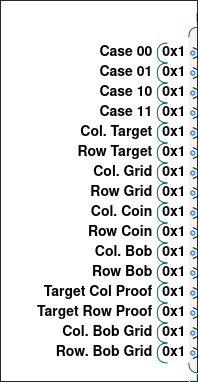
\includegraphics[width=0.8\linewidth]{image.png}
            \caption{Q-Bits}
            \label{fig:enter-label}
        \end{center}
    \end{wrapfigure}
    L'on dispose de 4 Q-bits représentant 4 cases (cf. \hyperref[sec:grid-2x2]{section 2.1}).
    \vspace{5mm}
    
    Les Q-bits \textbf{Col.Target} et \textbf{Row.Target} représentent la position de la case ciblée. Dans le cas d'une grille 4x4, target représentera premièrement la sous-grille dans laquelle se trouve la clé, puis dans un second temps la case dans laquelle ce trouve la clé. La concaténation des deux tirages de Target nous donnent les 4 bits de la position de la clé.
    
    \vspace{5mm}

    Les Q-bits \textbf{Col.Grid} et \textbf{Row.Grid} donnent la position de la sous-grille où le jeton doit être flip. Nous avons abitrairement choisi la sous grille en bas à gauche. Ainsi, Alice devra flip le coin en \textbf{11XY} où X est donné par \textbf{Row.Grid} et Y par \textbf{Col.Grid}.

    \vspace{5mm}

    De manière analogue, \textbf{Row.Coin} et \textbf{Col.Coin} représentent respectivement le bit \textbf{X} et \textbf{Y} de la case à la position \textbf{00XY} de la pièce à tourner.

    \vspace{5mm}

    Enfin, les Q-bits \textbf{Row.Bob.Grid} et \textbf{Col.Bob.Grid}, \textbf{Row.Bob} et \textbf{Col.Bob} donnent de les composantes X et Y des deux coins que Bob doit flip respectivement en bas à droite (\textbf{11XY}) et en haut à gauche (\textbf{00XY}).

    \vspace{5mm}
    Notez que les Q-bits \textbf{Target Col Proof} et \textbf{Target Row Proof} servent uniquement à vérifier la justesse de \textbf{Col.Bob.Grid} et \textbf{Row.Bob.Grid} lors du tirage de la sous-grille.
    De même, \textbf{Col.Target} et \textbf{Row.Target} sont mesurés pour vérifier la justesse de \textbf{Col.Bob} et \textbf{Row.Bob}.

    \vspace{10mm}
    Comme vu ci-dessus, le pattern est scalable à une grille 8x8. Pour celà, il nous faudra simplement une paire de Q-bits en plus représentant la position dans la 2e sous-grille, et le choix arbitraire d'un coin de l'échiquier.

    \section{Analyse mathématique}

    Analyse mathématique de la dernière partie de la grille 4x4. Nous avons choisi seulement la fin, car on y trouve le choix final de la case et on peut remarquer que la première partie est très similaire à celle-ci.
\begin{center}
    ========== PREPARE ========== \\

\[
    \begin{array}{l}
    |\psi_{0}\rangle = \left(
    \mathbbm{1} \oplus \mathbbm{1} \oplus \mathbbm{1} \oplus \mathbbm{1} \oplus \mathbbm{1} \oplus \mathbbm{1} \oplus H \oplus H \oplus H \oplus H \oplus H \oplus H 
    \right) |\ 000000000000\rangle \\
    
    |\psi_{0}\rangle = \frac{1}{8} \left(
    |000000000000\rangle + |000000000001\rangle + |000000000010\rangle + |000000000011\rangle \\ 
    + |000000000100\rangle + |000000000101\rangle + |000000000110\rangle + |000000000111\rangle \\
    + |000000001000\rangle + |000000001001\rangle + |000000001010\rangle + |000000001011\rangle \\
    + |000000001100\rangle + |000000001101\rangle + |000000001110\rangle + |000000001111\rangle + |000000010000\rangle \\
    + |000000010001\rangle + |000000010010\rangle + |000000010011\rangle + |000000010100\rangle \\
    + |000000010101\rangle + |000000010110\rangle + |000000010111\rangle + |000000011000\rangle + |000000011001\rangle \\
    + |000000011010\rangle + |000000011011\rangle + |000000011100\rangle + |000000011101\rangle \\
    + |000000011110\rangle + |000000011111\rangle + |000000100000\rangle + |000000100001\rangle \\
    + |000000100010\rangle + |000000100011\rangle + |000000100100\rangle + |000000100101\rangle \\ 
    + |000000100110\rangle + |000000100111\rangle + |000000101000\rangle + |000000101001\rangle \\
    + |000000101010\rangle + |000000101011\rangle + |000000101100\rangle + |000000101101\rangle +  |000000101110\rangle\\ 
    + |000000101111\rangle + |000000110000\rangle + |000000110001\rangle + |000000110010\rangle \\ 
    + |000000110011\rangle + |000000110100\rangle + |000000110101\rangle+ |000000110110\rangle + |000000110111\rangle \\ 
    + |000000111000\rangle + |000000111001\rangle + |000000111010\rangle + |000000111011\rangle \\
    + |000000111100\rangle + |000000111101\rangle + |000000111110\rangle + |000000111111\rangle \right)) \\ 
     \end{array}
    \]

    ========== PARITE TARGET (COIN) ========== \\

  \[
    \begin{array}{l}
    |\psi_{1}\rangle = \hat{c}\ |\ \psi_{0} \rangle\ (\( \color{blue}1e\ cnot\)) \\ 
    |\psi_{1}\rangle = \frac{1}{8} (
    |000000000000\rangle + |000000000001\rangle + |000\red{1}000000\red{1}0\rangle + |000\red{1}000000\red{1}1\rangle \\ 
    + |000000000100\rangle + |000000000101\rangle + |000\red{1}000001\red{1}0\rangle + |000\red{1}000001\red{1}1\rangle \\
    + |000000001000\rangle + |000000001001\rangle + |000\red{1}000010\red{1}0\rangle + |000\red{1}000010\red{1}1\rangle \\
    + |000000001100\rangle + |000000001101\rangle + |000\red{1}000011\red{1}0\rangle + |000\red{1}000011\red{1}1\rangle + |000000010000\rangle \\
    + |000000010001\rangle + |000\red{1}000100\red{1}0\rangle + |000\red{1}000100\red{1}1\rangle + |000000010100\rangle \\
    + |000000010101\rangle + |000\red{1}000101\red{1}0\rangle + |000\red{1}000101\red{1}1\rangle + |000000011000\rangle + |000000011001\rangle \\
    + |000\red{1}000110\red{1}0\rangle + |000\red{1}000110\red{1}1\rangle + |000000011100\rangle + |000000011101\rangle \\
    + |000\red{1}000111\red{1}0\rangle + |000\red{1}000111\red{1}1\rangle + |000000100000\rangle + |000000100001\rangle \\
    + |000\red{1}001000\red{1}0\rangle + |000\red{1}001000\red{1}1\rangle + |000000100100\rangle + |000000100101\rangle \\ 
    + |000\red{1}001001\red{1}0\rangle + |000\red{1}001001\red{1}1\rangle + |000000101000\rangle + |000000101001\rangle \\
    + |000\red{1}001010\red{1}0\rangle + |000\red{1}001010\red{1}1\rangle + |000000101100\rangle + |000000101101\rangle + |000\red{1}001011\red{1}0\rangle \\ 
    + |000\red{1}001011\red{1}1\rangle + |000000110000\rangle + |000000110001\rangle + |000\red{1}001100\red{1}0\rangle \\ 
    + |000\red{1}001100\red{1}1\rangle + |000000110100\rangle + |000000110101\rangle + |000\red{1}001101\red{1}0\rangle + |000\red{1}001101\red{1}1\rangle \\ 
    + |000000111000\rangle + |000000111001\rangle + |000\red{1}001110\red{1}0\rangle + |000\red{1}001110\red{1}1\rangle \\
    + |000000111100\rangle + |000000111101\rangle + |000\red{1}001111\red{1}0\rangle + |000\red{1}001111\red{1}1\rangle  ) \\
         \end{array}
    \]

    \[
    \begin{array}{l}
     |\psi_{2}\rangle = \hat{c}\ |\ \psi_{1} \rangle\ (\( \color{blue}2e\ cnot\)) \\ 
    |\psi_{2}\rangle = \frac{1}{8} (
    |000000000000\rangle + |000000000001\rangle + |000100000010\rangle + |000100000011\rangle \\ 
    + |000000000100\rangle + |000000000101\rangle + |000100000110\rangle + |000100000111\rangle \\
    + |000\red{1}0000\red{1}000\rangle + |000\red{1}0000\red{1}001\rangle + |000\red{0}0000\red{1}010\rangle + |000\red{0}0000\red{1}011\rangle \\
    + |000\red{1}0000\red{1}100\rangle + |000\red{1}0000\red{1}101\rangle + |000\red{0}0000\red{1}110\rangle + |000\red{0}0000\red{1}111\rangle + |000000010000\rangle \\
    + |000000010001\rangle + |000100010010\rangle + |000100010011\rangle + |000000010100\rangle \\
    + |000000010101\rangle + |000100010110\rangle + |000100010111\rangle + |000\red{1}0001\red{1}000\rangle + |000\red{1}0001\red{1}001\rangle \\
    + |000\red{0}0001\red{1}010\rangle + |000\red{0}0001\red{1}011\rangle + |000\red{1}0001\red{1}100\rangle + |000\red{1}0001\red{1}101\rangle \\
    + |000\red{0}0001\red{1}110\rangle + |000\red{0}0001\red{1}111\rangle + |000000100000\rangle + |000000100001\rangle \\
    + |000100100010\rangle + |000100100011\rangle + |000000100100\rangle + |000000100101\rangle \\ 
    + |000100100110\rangle + |000100100111\rangle + |000\red{1}0010\red{1}000\rangle + |000\red{1}0010\red{1}001\rangle \\
    + |000\red{0}0010\red{1}010\rangle + |000\red{0}0010\red{1}011\rangle + |000\red{1}0010\red{1}100\rangle + |000\red{1}0010\red{1}101\rangle  + |000\red{0}0010\red{1}110\rangle \\ 
    + |000\red{0}0010\red{1}111\rangle + |000000110000\rangle + |000000110001\rangle + |000100110010\rangle \\ 
    + |000100110011\rangle + |000000110100\rangle + |000000110101\rangle + |000100110110\rangle + |000100110111\rangle \\ 
    + |000\red{1}0011\red{1}000\rangle + |000\red{1}0011\red{1}001\rangle + |000\red{0}0011\red{1}010\rangle + |000\red{0}0011\red{1}011\rangle \\
    + |000\red{1}0011\red{1}100\rangle + |000\red{1}0011\red{1}101\rangle + |000\red{0}0011\red{1}110\rangle + |000\red{0}0011\red{1}111\rangle  ) \\
    \end{array}
    \]

    \[
    \begin{array}{l}
     |\psi_{3}\rangle = \hat{c}\ |\ \psi_{2} \rangle\ (\( \color{blue}3e\ cnot\)) \\ 
    |\psi_{3}\rangle = \frac{1}{8} (
    |000000000000\rangle + |000000000001\rangle + |000100000010\rangle + |000100000011\rangle \\ 
    + |00\red{1}000000\red{1}00\rangle + |00\red{1}000000\red{1}01\rangle + |00\red{1}100000\red{1}10\rangle + |00\red{1}100000\red{1}11\rangle \\
    + |000100001000\rangle + |000100001001\rangle + |000000001010\rangle + |000000001011\rangle \\
    + |00\red{1}100001\red{1}00\rangle + |00\red{1}100001\red{1}01\rangle + |00\red{1}000001\red{1}10\rangle + |00\red{1}000001\red{1}11\rangle + |000000010000\rangle \\
    + |000000010001\rangle + |000100010010\rangle + |000100010011\rangle + |00\red{1}000010\red{1}00\rangle \\
    + |00\red{1}000010\red{1}01\rangle + |00\red{1}100010\red{1}10\rangle + |00\red{1}100010\red{1}11\rangle + |000100011000\rangle + |000100011001\rangle \\
    + |000000011010\rangle + |000000011011\rangle + |00\red{1}100011\red{1}00\rangle + |00\red{1}100011\red{1}01\rangle \\
    + |00\red{1}000011\red{1}10\rangle + |00\red{1}000011\red{1}11\rangle + |000000100000\rangle + |000000100001\rangle \\
    + |000100100010\rangle + |000100100011\rangle + |00\red{1}000100\red{1}00\rangle + |00\red{1}000100\red{1}01\rangle \\ 
    + |00\red{1}100100\red{1}10\rangle + |00\red{1}100100\red{1}11\rangle + |000100101000\rangle + |000100101001\rangle \\
    + |000000101010\rangle + |000000101011\rangle + |00\red{1}100101\red{1}00\rangle + |00\red{1}100101\red{1}01\rangle  + |00\red{1}000101\red{1}10\rangle \\ 
    + |00\red{1}000101\red{1}11\rangle + |000000110000\rangle + |000000110001\rangle + |000100110010\rangle \\ 
    + |000100110011\rangle + |000000110100\rangle + |00\red{1}000110\red{1}01\rangle + |00\red{1}100110\red{1}10\rangle + |00\red{1}100110\red{1}11\rangle \\ 
    + |000100111000\rangle + |000100111001\rangle + |000000111010\rangle + |000000111011\rangle \\
    + |00\red{1}100111\red{1}00\rangle + |00\red{1}100111\red{1}01\rangle + |00\red{1}000111\red{1}10\rangle + |00\red{1}000111\red{1}11\rangle  ) \\
    \end{array}
    \]

      \[
    \begin{array}{l}
     |\psi_{4}\rangle = \hat{c}\ |\ \psi_{3} \rangle\ (\( \color{blue}4e\ cnot\)) \\ 
    |\psi_{4}\rangle = \frac{1}{8} (
    |000000000000\rangle + |000000000001\rangle + |000100000010\rangle + |000100000011\rangle \\ 
    + |001000000100\rangle + |001000000101\rangle + |001100000110\rangle + |001100000111\rangle \\
    + |00\red{1}10000\red{1}000\rangle + |00\red{1}10000\red{1}001\rangle + |00\red{1}00000\red{1}010\rangle + |00\red{1}00000\red{1}011\rangle \\
    + |00\red{0}10000\red{1}100\rangle + |00\red{0}10000\red{1}101\rangle + |00\red{0}00000\red{1}110\rangle + |00\red{0}00000\red{1}111\rangle + |000000010000\rangle \\
    + |000000010001\rangle + |000100010010\rangle + |000100010011\rangle + |001000010100\rangle \\
    + |001000010101\rangle + |001100010110\rangle + |001100010111\rangle + |00\red{1}10001\red{1}000\rangle + |00\red{1}10001\red{1}001\rangle \\
    + |00\red{1}00001\red{1}010\rangle + |00\red{1}00001\red{1}011\rangle + |00\red{0}10001\red{1}100\rangle + |00\red{0}10001\red{1}101\rangle \\
    + |00\red{0}00001\red{1}110\rangle + |00\red{0}00001\red{1}111\rangle + |000000100000\rangle + |000000100001\rangle \\
    + |000100100010\rangle + |000100100011\rangle + |001000100100\rangle + |001000100101\rangle \\ 
    + |001100100110\rangle + |001100100111\rangle + |00\red{1}10010\red{1}000\rangle + |00\red{1}10010\red{1}001\rangle \\
    + |00\red{1}00010\red{1}010\rangle + |00\red{1}00010\red{1}011\rangle + |00\red{0}10010\red{1}100\rangle + |00\red{0}10010\red{1}101\rangle  + |00\red{0}00010\red{1}110\rangle \\ 
    + |00\red{0}00010\red{1}111\rangle + |000000110000\rangle + |000000110001\rangle + |000100110010\rangle \\ 
    + |000100110011\rangle + |000000110100\rangle + |001000110101\rangle + |001100110110\rangle + |001100110111\rangle \\ 
    + |00\red{1}10011\red{1}000\rangle + |00\red{1}10011\red{1}001\rangle + |00\red{1}00011\red{1}010\rangle + |00\red{1}00011\red{1}011\rangle \\
    + |00\red{0}10011\red{1}100\rangle + |00\red{0}10011\red{1}101\rangle + |00\red{0}00011\red{1}110\rangle + |00\red{0}00011\red{1}111\rangle  ) \\
    \end{array}
    \]

    \[
    \begin{array}{l}
     |\psi_{5}\rangle = \hat{c}\ |\ \psi_{4} \rangle\ (\( \color{blue}5e\ cnot\)) \\ 
    |\psi_{5}\rangle = \frac{1}{8} (
    |000000000000\rangle + |000000000001\rangle + |000100000010\rangle + |000100000011\rangle \\ 
    + |001000000100\rangle + |001000000101\rangle + |001100000110\rangle + |001100000111\rangle \\
    + |001100001000\rangle + |001100001001\rangle + |001000001010\rangle + |001000001011\rangle \\
    + |000100001100\rangle + |000100001101\rangle + |000000001110\rangle + |000000001111\rangle + |000000010000\rangle \\
    + |000\red{1}000\red{1}0001\rangle + |000\red{0}000\red{1}0010\rangle + |000\red{0}000\red{1}0011\rangle + |001\red{0}000\red{1}0100\rangle \\
    + |001\red{1}000\red{1}0101\rangle + |001\red{0}000\red{1}0110\rangle + |001\red{0}000\red{1}0111\rangle + |001\red{0}000\red{1}1000\rangle + |001\red{0}000\red{1}1001\rangle \\
    + |001\red{1}000\red{1}1010\rangle + |001\red{1}000\red{1}1011\rangle + |000\red{0}000\red{1}1100\rangle + |000\red{0}000\red{1}1101\rangle \\
    + |000\red{1}000\red{1}1110\rangle + |000\red{1}000\red{1}1111\rangle + |000000100000\rangle + |000000100001\rangle \\
    + |000100100010\rangle + |000100100011\rangle + |001000100100\rangle + |001000100101\rangle \\ 
    + |001100100110\rangle + |001100100111\rangle + |001100101000\rangle + |001100101001\rangle \\
    + |001000101010\rangle + |001000101011\rangle + |000100101100\rangle + |000100101101\rangle  + |000000101110\rangle \\ 
    + |000000101111\rangle + |000\red{1}001\red{1}0000\rangle + |000\red{1}001\red{1}0001\rangle + |000\red{0}001\red{1}0010\rangle \\ 
    + |000\red{0}001\red{1}0011\rangle + |000\red{1}001\red{1}0100\rangle + |001\red{1}001\red{1}0101\rangle + |001\red{0}001\red{1}0110\rangle + |001\red{0}001\red{1}0111\rangle \\ 
    + |001\red{0}001\red{1}1000\rangle + |001\red{0}001\red{1}1001\rangle + |001\red{1}001\red{1}1010\rangle + |001000111011\rangle \\
    + |000\red{0}001\red{1}1100\rangle + |000\red{0}001\red{1}1101\rangle + |000\red{1}001\red{1}1110\rangle + |000\red{1}001\red{1}1111\rangle  ) \\
    \end{array}
    \]
    
    \[
    \begin{array}{l}
     |\psi_{6}\rangle = \hat{c}\ |\ \psi_{5} \rangle\ (\( \color{blue}6e\ cnot\)) \\ 
    |\psi_{6}\rangle = \frac{1}{8} (
    |000000000000\rangle + |000000000001\rangle + |000100000010\rangle + |000100000011\rangle \\ 
    + |001000000100\rangle + |001000000101\rangle + |001100000110\rangle + |001100000111\rangle \\
    + |001100001000\rangle + |001100001001\rangle + |001000001010\rangle + |001000001011\rangle \\
    + |000100001100\rangle + |000100001101\rangle + |000000001110\rangle + |000000001111\rangle + |000000010000\rangle \\
    + |000100010001\rangle + |000000010010\rangle + |000000010011\rangle + |001000010100\rangle \\
    + |001100010101\rangle + |001000010110\rangle + |001000010111\rangle + |001000011000\rangle + |001000011001\rangle \\
    + |001100011010\rangle + |001100011011\rangle + |000000011100\rangle + |000000011101\rangle \\
    + |000100011110\rangle + |000100011111\rangle + |00\red{1}000\red{1}00000\rangle + |00\red{1}000\red{1}00001\rangle \\
    + |00\red{1}100\red{1}00010\rangle + |00\red{1}100\red{1}00011\rangle + |00\red{0}000\red{1}00100\rangle + |00\red{0}000\red{1}00101\rangle \\ 
    + |00\red{0}100\red{1}00110\rangle + |00\red{0}100\red{1}00111\rangle + |00\red{0}100\red{1}01000\rangle + |00\red{0}100\red{1}01001\rangle \\
    + |00\red{0}000\red{1}01010\rangle + |00\red{0}000\red{1}01011\rangle + |00\red{1}100\red{1}01100\rangle + |00\red{1}100\red{1}01101\rangle  + |00\red{1}000\red{1}01110\rangle \\ 
    + |00\red{1}000\red{1}01111\rangle + |00\red{1}100\red{1}10000\rangle + |00\red{1}100\red{1}10001\rangle + |00\red{1}000\red{1}10010\rangle \\ 
    + |00\red{1}000\red{1}10011\rangle + |00\red{1}100\red{1}10100\rangle + |00\red{0}100\red{1}10101\rangle + |00\red{0}000\red{1}10110\rangle + |00\red{0}000\red{1}10111\rangle \\ 
    + |00\red{0}000\red{1}11000\rangle + |00\red{0}000\red{1}11001\rangle + |00\red{0}100\red{1}11010\rangle + |00\red{0}000\red{1}11011\rangle \\
    + |00\red{1}000\red{1}11100\rangle + |00\red{1}000\red{1}11101\rangle + |00\red{1}100\red{1}11110\rangle + |00\red{1}100\red{1}11111\rangle  ) \\
    \end{array}
    \]

    ========== FLIP COIN (TOP LEFT) ========== \\

     \begin{array}{l}
     |\psi_{7}\rangle = \hat{c}\ |\ \psi_{6} \rangle\ (\( \color{blue}7e\ cnot\)) \\ 
    |\psi_{7}\rangle = \frac{1}{8} (
    |000000000000\rangle + |000000000001\rangle + |000100000010\rangle + |000100000011\rangle \\ 
    + |001000000100\rangle + |001000000101\rangle + |00\red{11}0000\red{1}110\rangle + |00\red{11}0000\red{1}111\rangle \\
    + |00\red{11}0000\red{0}000\rangle + |00\red{11}0000\red{0}001\rangle + |001000001010\rangle + |001000001011\rangle \\
    + |000100001100\rangle + |000100001101\rangle + |000000001110\rangle + |000000001111\rangle + |000000010000\rangle \\
    + |000100010001\rangle + |000000010010\rangle + |000000010011\rangle + |001000010100\rangle \\
    + |00\red{11}0001\red{1}101\rangle + |001000010110\rangle + |001000010111\rangle + |001000011000\rangle + |001000011001\rangle \\
    + |00\red{11}0001\red{0}010\rangle + |00\red{11}0001\red{0}011\rangle + |000000011100\rangle + |000000011101\rangle \\
    + |000100011110\rangle + |000100011111\rangle + |001000100000\rangle + |001000100001\rangle \\
    + |00\red{11}0010\red{1}010\rangle + |00\red{11}0010\red{1}011\rangle + |000000100100\rangle + |000000100101\rangle \\ 
    + |000100100110\rangle + |000100100111\rangle + |000100101000\rangle + |000100101001\rangle \\
    + |000000101010\rangle + |000000101011\rangle + |00\red{11}0010\red{0}100\rangle + |00\red{11}0010\red{0}101\rangle + |001000101110\rangle \\ 
    + |001000101111\rangle + |00\red{11}0011\red{1}000\rangle + |00\red{11}0011\red{1}001\rangle + |001000110010\rangle \\ 
    + |001000110011\rangle + |00\red{11}0011\red{1}100\rangle + |000100110101\rangle + |000000110110\rangle + |000000110111\rangle \\ 
    + |000000111000\rangle + |000000111001\rangle + |000100111010\rangle + |000000111011\rangle \\
    + |001000111100\rangle + |001000111101\rangle + |00\red{11}0011\red{0}110\rangle + |00\red{11}0011\red{0}111\rangle  ) \\
    \end{array}
    \]

    \[
     \begin{array}{l}
     |\psi_{8}\rangle = \hat{n}\ |\ \psi_{7} \rangle\ (\( \color{blue}1e\ not\)) \\ 
    |\psi_{8}\rangle = \frac{1}{8} (
    |000\red{1}00000000\rangle + |000\red{1}00000001\rangle + |000\red{0}00000010\rangle + |000\red{0}00000011\rangle \\ 
    + |001\red{1}00000100\rangle + |001\red{1}00000101\rangle + |001\red{0}00001110\rangle + |001\red{0}00001111\rangle \\
    + |001\red{0}00000000\rangle + |001\red{0}00000001\rangle + |001\red{1}00001010\rangle + |001\red{1}00001011\rangle \\
    + |000\red{0}00001100\rangle + |000\red{0}00001101\rangle + |000\red{1}00001110\rangle + |000\red{1}00001111\rangle + |000\red{1}00010000\rangle \\
    + |000\red{0}00010001\rangle + |000\red{1}00010010\rangle + |000\red{1}00010011\rangle + |001\red{1}00010100\rangle \\
    + |001\red{0}00011101\rangle + |001\red{1}00010110\rangle + |001\red{1}00010111\rangle + |001\red{1}00011000\rangle + |001\red{1}00011001\rangle \\
    + |001\red{0}00010010\rangle + |001\red{0}00010011\rangle + |000\red{1}00011100\rangle + |000\red{1}00011101\rangle \\
   
    
    + |000\red{1}00011110\rangle + |000\red{1}00011111\rangle + |001\red{1}00100000\rangle + |001\red{1}00100001\rangle \\
    + |001\red{1}00101010\rangle + |001\red{1}00101011\rangle + |000\red{1}00100100\rangle + |000\red{1}00100101\rangle \\ 
    + |000\red{1}00100110\rangle + |000\red{1}00100111\rangle + |000\red{1}00101000\rangle + |000\red{1}00101001\rangle \\
    + |000\red{1}00101010\rangle + |000\red{1}00101011\rangle + |001\red{1}00100100\rangle + |001\red{1}00100101\rangle + |001\red{1}00101110\rangle \\ 
    + |001100101111\rangle + |001100111000\rangle + |001100111001\rangle + |001100110010\rangle \\ 
    + |001100110011\rangle + |001100111100\rangle + |000100110101\rangle + |000100110110\rangle + |000100110111\rangle \\ 
    + |000100111000\rangle + |000100111001\rangle + |000100111010\rangle + |000100111011\rangle \\
    + |001100111100\rangle + |001100111101\rangle + |001100110110\rangle + |001100110111\rangle  ) \\
    \end{array}
    \]

     \[
     \begin{array}{l}
     |\psi_{9}\rangle = \hat{c}\ |\ \psi_{8} \rangle\ (\( \color{blue}8e\ cnot\)) \\ 
    |\psi_{9}\rangle = \frac{1}{8} (
    |000100000000\rangle + |000100000001\rangle + |000000000010\rangle + |000000000011\rangle \\ 
    + |00\red{11}00000\red{0}00\rangle + |00\red{11}00000\red{0}01\rangle + |001000001110\rangle + |001000001111\rangle \\
    + |001000000000\rangle + |001000000001\rangle + |00\red{11}00001\red{1}10\rangle + |00\red{11}00001\red{1}11\rangle \\
    + |000000001100\rangle + |000000001101\rangle + |000100001110\rangle + |000100001111\rangle + |000100010000\rangle \\
    + |000000010001\rangle + |000100010010\rangle + |000100010011\rangle + |00\red{11}00010\red{0}00\rangle \\
    + |001000011101\rangle + |00\red{11}00010\red{0}10\rangle + |00\red{11}00010\red{0}11\rangle + |00\red{11}00011\red{1}00\rangle + |00\red{11}00011\red{1}01\rangle \\
    + |001000010010\rangle + |001000010011\rangle + |000100011100\rangle + |000100011101\rangle \\
    + |000100011110\rangle + |000100011111\rangle + |00\red{11}00100\red{1}00\rangle + |00\red{11}00100\red{1}01\rangle \\
    + |00\red{11}00101\red{1}10\rangle + |00\red{11}00101\red{1}11\rangle + |000100100100\rangle + |000100100101\rangle \\ 
    + |000100100110\rangle + |000100100111\rangle + |000100101000\rangle + |000100101001\rangle \\
    + |000100101010\rangle + |000100101011\rangle + |00\red{11}00100\red{0}00\rangle + |00\red{11}00100\red{0}01\rangle + |00\red{11}00101\red{0}10\rangle \\ 
    + |00\red{11}00101\red{0}11\rangle + |00\red{11}00111\red{1}00\rangle + |00\red{11}00111\red{1}01\rangle + |00\red{11}00110\red{1}10\rangle \\ 
    + |00\red{11}00110\red{1}11\rangle + |00\red{11}00111\red{0}00\rangle + |000100110101\rangle + |000100110110\rangle + |000100110111\rangle \\ 
    + |000100111000\rangle + |000100111001\rangle + |000100111010\rangle + |000100111011\rangle \\
    + |00\red{11}00111\red{0}00\rangle + |00\red{11}00111\red{0}01\rangle + |00\red{11}00110\red{0}10\rangle + |00\red{11}00110\red{0}11\rangle  ) \\
    \end{array}
    \]

    \[
     \begin{array}{l}
     |\psi_{10}\rangle = \hat{n}\ |\ \psi_{9} \rangle\ (\( \color{blue}2e\ not\)) \\ 
    |\psi_{10}\rangle = \frac{1}{8} (
    |000\red{0}00000000\rangle + |000\red{0}00000001\rangle + |000\red{1}00000010\rangle + |000\red{1}00000011\rangle \\ 
    + |001\red{0}00000000\rangle + |001\red{0}00000001\rangle + |001\red{1}00001110\rangle + |001\red{1}00001111\rangle \\
    + |001\red{1}00000000\rangle + |001\red{1}00000001\rangle + |001\red{0}00001110\rangle + |001\red{0}00001111\rangle \\
    + |000\red{1}00001100\rangle + |000\red{1}00001101\rangle + |000\red{0}00001110\rangle + |000\red{0}00001111\rangle + |000\red{0}00010000\rangle \\
    + |000\red{1}00010001\rangle + |000\red{0}00010010\rangle + |000\red{0}00010011\rangle + |001\red{0}00010000\rangle \\
    + |001\red{1}00011101\rangle + |001\red{0}00010010\rangle + |001\red{0}00010011\rangle + |001\red{0}00011100\rangle + |001\red{0}00011101\rangle \\
    + |001\red{1}00010010\rangle + |001\red{1}00010011\rangle + |000\red{0}00011100\rangle + |000\red{0}00011101\rangle \\
    + |000\red{0}00011110\rangle + |000\red{0}00011111\rangle + |001\red{0}00100100\rangle + |001\red{0}00100101\rangle \\
    + |001\red{0}00101110\rangle + |001\red{0}00101111\rangle + |000\red{0}00100100\rangle + |000\red{0}00100101\rangle \\ 
    + |000\red{0}00100110\rangle + |000\red{0}00100111\rangle + |000\red{0}00101000\rangle + |000\red{0}00101001\rangle \\
    + |000\red{0}00101010\rangle + |000\red{0}00101011\rangle + |001\red{0}00100000\rangle + |001\red{0}00100001\rangle + |001\red{0}00101010\rangle \\ 
    + |001000101011\rangle + |001000111100\rangle + |001000111101\rangle + |001000110110\rangle \\ 
    + |001000110111\rangle + |001000111000\rangle + |000000110101\rangle + |000000110110\rangle + |000000110111\rangle \\ 
    + |000000111000\rangle + |000000111001\rangle + |000000111010\rangle + |000000111011\rangle \\
    + |001000111000\rangle + |001000111001\rangle + |001000110010\rangle + |001000110011\rangle  ) \\
    \end{array}
    \]

      \[
     \begin{array}{l}
     |\psi_{11}\rangle = \hat{n}\ |\ \psi_{10} \rangle\ (\( \color{blue}3e\ not\)) \\ 
    |\psi_{11}\rangle = \frac{1}{8} (
    |00\red{1}000000000\rangle + |00\red{1}000000001\rangle + |00\red{1}100000010\rangle + |00\red{1}100000011\rangle \\ 
    + |00\red{0}000000000\rangle + |00\red{0}000000001\rangle + |00\red{0}100001110\rangle + |00\red{0}100001111\rangle \\
    + |00\red{0}100000000\rangle + |00\red{0}100000001\rangle + |00\red{0}000001110\rangle + |00\red{0}000001111\rangle \\
    + |00\red{1}100001100\rangle + |00\red{1}100001101\rangle + |00\red{1}000001110\rangle + |00\red{1}000001111\rangle + |00\red{1}000010000\rangle \\
    + |00\red{1}100010001\rangle + |00\red{1}000010010\rangle + |00\red{1}000010011\rangle + |00\red{0}000010000\rangle \\
    + |00\red{0}100011101\rangle + |00\red{0}000010010\rangle + |00\red{0}000010011\rangle + |00\red{0}000011100\rangle + |00\red{0}000011101\rangle \\
    + |00\red{0}100010010\rangle + |00\red{0}100010011\rangle + |00\red{1}000011100\rangle + |00\red{1}000011101\rangle \\
    + |00\red{1}000011110\rangle + |00\red{1}000011111\rangle + |00\red{0}000100100\rangle + |00\red{0}000100101\rangle \\
    + |000000101110\rangle + |000000101111\rangle + |001000100100\rangle + |001000100101\rangle \\ 
    + |001000100110\rangle + |001000100111\rangle + |001000101000\rangle + |001000101001\rangle \\
    + |001000101010\rangle + |001000101011\rangle + |000000100000\rangle + |000000100001\rangle + |000000101010\rangle \\ 
    + |000000101011\rangle + |000000111100\rangle + |000000111101\rangle + |000000110110\rangle \\ 
    + |000000110111\rangle + |000000111000\rangle + |001000110101\rangle + |001000110110\rangle + |001000110111\rangle \\ 
    + |001000111000\rangle + |001000111001\rangle + |001000111010\rangle + |001000111011\rangle \\
    + |000000111000\rangle + |000000111001\rangle + |000000110010\rangle + |000000110011\rangle  ) \\
    \end{array}
    \]

     \[
     \begin{array}{l}
     |\psi_{12}\rangle = \hat{c}\ |\ \psi_{11} \rangle\ (\( \color{blue}9e\ cnot\)) \\ 
    |\psi_{12}\rangle = \frac{1}{8} (
    |001000000000\rangle + |001000000001\rangle + |00\red{11}000000\red{0}0\rangle + |00\red{11}000000\red{0}1\rangle \\ 
    + |000000000000\rangle + |000000000001\rangle + |000100001110\rangle + |000100001111\rangle \\
    + |000100000000\rangle + |000100000001\rangle + |000000001110\rangle + |000000001111\rangle \\
    + |00\red{11}000011\red{1}0\rangle + |00\red{11}000011\red{1}1\rangle + |001000001110\rangle + |001000001111\rangle + |001000010000\rangle \\
    + |00\red{11}000100\red{1}1\rangle + |001000010010\rangle + |001000010011\rangle + |000000010000\rangle \\
    + |000100011101\rangle + |000000010010\rangle + |000000010011\rangle + |000000011100\rangle + |000000011101\rangle \\
    + |000100010010\rangle + |000100010011\rangle + |001000011100\rangle + |001000011101\rangle \\
    + |001000011110\rangle + |001000011111\rangle + |000000100100\rangle + |000000100101\rangle \\
    + |000000101110\rangle + |000000101111\rangle + |001000100100\rangle + |001000100101\rangle \\ 
    + |001000100110\rangle + |001000100111\rangle + |001000101000\rangle + |001000101001\rangle \\
    + |001000101010\rangle + |001000101011\rangle + |000000100000\rangle + |000000100001\rangle + |000000101010\rangle \\ 
    + |000000101011\rangle + |000000111100\rangle + |000000111101\rangle + |000000110110\rangle \\ 
    + |000000110111\rangle + |000000111000\rangle + |001000110101\rangle + |001000110110\rangle + |001000110111\rangle \\ 
    + |001000111000\rangle + |001000111001\rangle + |001000111010\rangle + |001000111011\rangle \\
    + |000000111000\rangle + |000000111001\rangle + |000000110010\rangle + |000000110011\rangle  ) \\
    \end{array}
    \]

     \[
     \begin{array}{l}
     |\psi_{13}\rangle = \hat{n}\ |\ \psi_{12} \rangle\ (\( \color{blue}4e\ not\)) \\ 
    |\psi_{13}\rangle = \frac{1}{8} (
    |00\red{0}000000000\rangle + |00\red{0}000000001\rangle + |00\red{0}100000000\rangle + |00\red{0}100000001\rangle \\ 
    + |00\red{1}000000000\rangle + |00\red{1}000000001\rangle + |00\red{1}100001110\rangle + |00\red{1}100001111\rangle \\
    + |00\red{1}100000000\rangle + |00\red{1}100000001\rangle + |00\red{1}000001110\rangle + |00\red{1}000001111\rangle \\
    + |00\red{0}100001110\rangle + |00\red{0}100001111\rangle + |00\red{0}000001110\rangle + |00\red{0}000001111\rangle + |00\red{0}000010000\rangle \\
    + |00\red{0}100010011\rangle + |00\red{0}000010010\rangle + |00\red{0}000010011\rangle + |00\red{1}000010000\rangle \\
    + |00\red{1}100011101\rangle + |00\red{1}000010010\rangle + |00\red{1}000010011\rangle + |00\red{1}000011100\rangle + |00\red{1}000011101\rangle \\
    + |00\red{1}100010010\rangle + |00\red{1}100010011\rangle + |00\red{0}000011100\rangle + |00\red{0}000011101\rangle \\
    + |00\red{0}000011110\rangle + |00\red{0}000011111\rangle + |00\red{1}000100100\rangle + |00\red{1}000100101\rangle \\
    + |001000101110\rangle + |001000101111\rangle + |000000100100\rangle + |000000100101\rangle \\ 
    + |000000100110\rangle + |000000100111\rangle + |000000101000\rangle + |000000101001\rangle \\
    + |000000101010\rangle + |000000101011\rangle + |001000100000\rangle + |001000100001\rangle + |001000101010\rangle \\ 
    + |001000101011\rangle + |001000111100\rangle + |001000111101\rangle + |001000110110\rangle \\ 
    + |001000110111\rangle + |001000111000\rangle + |000000110101\rangle + |000000110110\rangle + |000000110111\rangle \\ 
    + |000000111000\rangle + |000000111001\rangle + |000000111010\rangle + |000000111011\rangle \\
    + |001000111000\rangle + |001000111001\rangle + |001000110010\rangle + |001000110011\rangle  ) \\
    \end{array}
    \]

    \[
     \begin{array}{l}
     |\psi_{14}\rangle = \hat{n}\ |\ \psi_{13} \rangle\ (\( \color{blue}5e\ et\ 6e\ not\)) \\ 
    |\psi_{14}\rangle = \frac{1}{8} (
    |00\red{11}00000000\rangle + |00\red{11}00000001\rangle + |00\red{10}00000000\rangle + |00\red{10}00000001\rangle \\ 
    + |00\red{01}00000000\rangle + |00\red{01}00000001\rangle + |00\red{00}00001110\rangle + |00\red{00}00001111\rangle \\
    + |00\red{00}00000000\rangle + |00\red{00}00000001\rangle + |00\red{01}00001110\rangle + |00\red{01}00001111\rangle \\
    + |00\red{10}00001110\rangle + |00\red{10}00001111\rangle + |00\red{11}00001110\rangle + |00\red{11}00001111\rangle + |00\red{11}00010000\rangle \\
    + |00\red{10}00010011\rangle + |00\red{11}00010010\rangle + |00\red{11}00010011\rangle + |00\red{01}00010000\rangle \\
    + |00\red{00}00011101\rangle + |00\red{01}00010010\rangle + |00\red{01}00010011\rangle + |00\red{01}00011100\rangle + |00\red{01}00011101\rangle \\
    + |00\red{00}00010010\rangle + |00\red{00}00010011\rangle + |00\red{11}00011100\rangle + |00\red{11}00011101\rangle \\
    + |00\red{11}00011110\rangle + |00\red{11}00011111\rangle + |00\red{01}00100100\rangle + |00\red{01}00100101\rangle \\
    + |000100101110\rangle + |000100101111\rangle + |001100100100\rangle + |001100100101\rangle \\ 
    + |001100100110\rangle + |001100100111\rangle + |001100101000\rangle + |001100101001\rangle \\
    + |001100101010\rangle + |001100101011\rangle + |000100100000\rangle + |000100100001\rangle + |000100101010\rangle \\ 
    + |000100101011\rangle + |000100111100\rangle + |000100111101\rangle + |000100110110\rangle \\ 
    + |000100110111\rangle + |000100111000\rangle + |001100110101\rangle + |001100110110\rangle + |001100110111\rangle \\ 
    + |001100111000\rangle + |001100111001\rangle + |001100111010\rangle + |001100111011\rangle \\
    + |000100111000\rangle + |000100111001\rangle + |000100110010\rangle + |000100110011\rangle  ) \\
    \end{array}
    \]

     \[
     \begin{array}{l}
     |\psi_{15}\rangle = \hat{c}\ |\ \psi_{14} \rangle\ (\( \color{blue}10e\ cnot\)) \\ 
    |\psi_{15}\rangle = \frac{1}{8} (
    |00\red{11}0000000\red{1}\rangle + |00\red{11}0000000\red{0}\rangle + |001000000000\rangle + |001000000001\rangle \\ 
    + |000100000000\rangle + |000100000001\rangle + |000000001110\rangle + |000000001111\rangle \\
    + |000000000000\rangle + |000000000001\rangle + |000100001110\rangle + |000100001111\rangle \\
    + |001000001110\rangle + |001000001111\rangle + |00\red{11}0000111\red{1}\rangle + |00\red{11}0000111\red{0}\rangle + |00\red{11}0001000\red{1}\rangle \\
    + |001000010011\rangle + |00\red{11}0001001\red{1}\rangle + |00\red{11}0001001\red{0}\rangle + |000100010000\rangle \\
    + |000000011101\rangle + |000100010010\rangle + |000100010011\rangle + |000100011100\rangle + |000100011101\rangle \\
    + |000000010010\rangle + |000000010011\rangle + |00\red{11}0001110\red{1}\rangle + |00\red{11}0001110\red{0}\rangle \\
    + |00\red{11}0001111\red{1}\rangle + |00\red{11}0001111\red{0}\rangle + |000100100100\rangle + |000100100101\rangle \\
    + |000100101110\rangle + |000100101111\rangle + |00\red{11}0010010\red{1}\rangle + |00\red{11}0010010\red{0}\rangle \\ 
    + |00\red{11}0010011\red{1}\rangle + |00\red{11}0010011\red{0}\rangle + |00\red{11}0010100\red{1}\rangle + |00\red{11}0010100\red{0}\rangle \\
    + |00\red{11}0010101\red{1}\rangle + |00\red{11}0010101\red{0}\rangle + |000100100000\rangle + |000100100001\rangle + |000100101010\rangle \\ 
    + |000100101011\rangle + |000100111100\rangle + |000100111101\rangle + |000100110110\rangle \\ 
    + |000100110111\rangle + |000100111000\rangle + |00\red{11}0011010\red{0}\rangle + |00\red{11}0011011\red{1}\rangle + |00\red{11}0011011\red{0}\rangle \\ 
    + |00\red{11}0011100\red{1}\rangle + |00\red{11}0011100\red{0}\rangle + |00\red{11}0011101\red{1}\rangle + |00\red{11}0011101\red{0}\rangle \\
    + |000100111000\rangle + |000100111001\rangle + |000100110010\rangle + |000100110011\rangle  ) \\
    \end{array}
    \]

    \[
     \begin{array}{l}
     |\psi_{16}\rangle = \hat{n}\ |\ \psi_{15} \rangle\ (\( \color{blue}7e\ et\ 8e\ not\)) \\ 
    |\psi_{16}\rangle = \frac{1}{8} (
    |00\red{00}00000001\rangle + |00\red{00}00000000\rangle + |00\red{01}00000000\rangle + |00\red{01}00000001\rangle \\ 
    + |00\red{10}00000000\rangle + |00\red{10}00000001\rangle + |00\red{11}00001110\rangle + |00\red{11}00001111\rangle \\
    + |00\red{11}00000000\rangle + |00\red{11}00000001\rangle + |00\red{10}00001110\rangle + |00\red{10}00001111\rangle \\
    + |00\red{01}00001110\rangle + |00\red{01}00001111\rangle + |00\red{00}00001111\rangle + |00\red{00}00001110\rangle + |00\red{00}00010001\rangle \\
    + |00\red{01}00010011\rangle + |00\red{00}00010011\rangle + |00\red{00}00010010\rangle + |00\red{10}00010000\rangle \\
    + |00\red{11}00011101\rangle + |00\red{10}00010010\rangle + |00\red{10}00010011\rangle + |00\red{10}00011100\rangle + |00\red{10}00011101\rangle \\
    + |00\red{11}00010010\rangle + |00\red{11}00010011\rangle + |00\red{00}00011101\rangle + |00\red{00}00011100\rangle \\
    + |00\red{00}00011111\rangle + |00\red{00}00011110\rangle + |00\red{10}00100100\rangle + |00\red{10}00100101\rangle \\
    + |001000101110\rangle + |001000101111\rangle + |000000100101\rangle + |000000100100\rangle \\ 
    + |000000100111\rangle + |000000100110\rangle + |000000101001\rangle + |000000101000\rangle \\
    + |000000101011\rangle + |000000101010\rangle + |001000100000\rangle + |001000100001\rangle + |001000101010\rangle \\ 
    + |001000101011\rangle + |001000111100\rangle + |001000111101\rangle + |001000110110\rangle \\ 
    + |001000110111\rangle + |001000111000\rangle + |000000110100\rangle + |000000110111\rangle + |000000110110\rangle \\ 
    + |000000111001\rangle + |000000111000\rangle + |000000111011\rangle + |000000111010\rangle \\
    + |001000111000\rangle + |001000111001\rangle + |001000110010\rangle + |001000110011\rangle  ) \\
    \end{array}
    \]

    ========== BOB READS ========== \\

    \[
     \begin{array}{l}
     |\psi_{17}\rangle = \hat{c}\ |\ \psi_{16} \rangle\ (\( \color{blue}11e\ cnot\)) \\ 
    |\psi_{17}\rangle = \frac{1}{8} (
    |000000000001\rangle + |000000000000\rangle + |000100000000\rangle + |000100000001\rangle \\ 
    + |001000000000\rangle + |001000000001\rangle + |0\red{1}11000011\red{1}0\rangle + |0\red{1}11000011\red{1}1\rangle \\
    + |001100000000\rangle + |001100000001\rangle + |0\red{1}10000011\red{1}0\rangle + |0\red{1}10000011\red{1}1\rangle \\
    + |0\red{1}01000011\red{1}0\rangle + |0\red{1}01000011\red{1}1\rangle + |0\red{1}00000011\red{1}1\rangle + |0\red{1}00000011\red{1}0\rangle + |000000010001\rangle \\
    + |0\red{1}01000100\red{1}1\rangle + |0\red{1}00000100\red{1}1\rangle + |0\red{1}00000100\red{1}0\rangle + |001000010000\rangle \\
    + |001100011101\rangle + |0\red{1}10000100\red{1}0\rangle + |0\red{1}10000100\red{1}1\rangle + |001000011100\rangle + |001000011101\rangle \\
    + |0\red{1}11000100\red{1}0\rangle + |0\red{1}11000100\red{1}1\rangle + |000000011101\rangle + |000000011100\rangle \\
    + |0\red{1}00000111\red{1}1\rangle + |0\red{1}00000111\red{1}0\rangle + |001000100100\rangle + |001000100101\rangle \\
    + |0\red{1}10001011\red{1}0\rangle + |0\red{1}10001011\red{1}1\rangle + |000000100101\rangle + |000000100100\rangle \\ 
    + |0\red{1}00001001\red{1}1\rangle + |0\red{1}00001001\red{1}0\rangle + |000000101001\rangle + |000000101000\rangle \\
    + |0\red{1}00001010\red{1}1\rangle + |0\red{1}00001010\red{1}0\rangle + |001000100000\rangle + |001000100001\rangle + |0\red{1}10001010\red{1}0\rangle \\ 
    + |0\red{1}10001010\red{1}1\rangle + |001000111100\rangle + |001000111101\rangle + |0\red{1}10001101\red{1}0\rangle \\ 
    + |0\red{1}10001101\red{1}1\rangle + |001000111000\rangle + |000000110100\rangle + |0\red{1}00001101\red{1}1\rangle + |0\red{1}00001101\red{1}0\rangle \\ 
    + |000000111001\rangle + |000000111000\rangle + |0\red{1}00001110\red{1}1\rangle + |0\red{1}00001110\red{1}0\rangle \\
    + |001000111000\rangle + |001000111001\rangle + |0\red{1}10001100\red{1}0\rangle + |0\red{1}10001100\red{1}1\rangle  ) \\
    \end{array}
    \]

    \[
     \begin{array}{l}
     |\psi_{18}\rangle = \hat{c}\ |\ \psi_{17} \rangle\ (\( \color{blue}12e\ cnot\)) \\ 
    |\psi_{18}\rangle = \frac{1}{8} (
    |000000000001\rangle + |000000000000\rangle + |000100000000\rangle + |000100000001\rangle \\ 
    + |001000000000\rangle + |001000000001\rangle + |0\red{0}110000\red{1}110\rangle + |0\red{0}110000\red{1}111\rangle \\
    + |001100000000\rangle + |001100000001\rangle + |0\red{0}100000\red{1}110\rangle + |0\red{0}100000\red{1}111\rangle \\
    + |0\red{0}010000\red{1}110\rangle + |0\red{0}010000\red{1}111\rangle + |0\red{0}000000\red{1}111\rangle + |0\red{0}000000\red{1}110\rangle + |000000010001\rangle \\
    + |010100010011\rangle + |010000010011\rangle + |010000010010\rangle + |001000010000\rangle \\
    + |0\red{1}110001\red{1}101\rangle + |011000010010\rangle + |011000010011\rangle + |0\red{1}100001\red{1}100\rangle + |0\red{1}100001\red{1}101\rangle \\
    + |011100010010\rangle + |011100010011\rangle + |0\red{1}000001\red{1}101\rangle + |0\red{1}000001\red{1}100\rangle \\
    + |0\red{0}000001\red{1}111\rangle + |0\red{0}000001\red{1}110\rangle + |001000100100\rangle + |001000100101\rangle \\
    + |0\red{0}100010\red{1}110\rangle + |0\red{0}100010\red{1}111\rangle + |000000100101\rangle + |000000100100\rangle \\ 
    + |010000100111\rangle + |010000100110\rangle + |0\red{1}000010\red{1}001\rangle + |0\red{1}000010\red{1}000\rangle \\
    + |0\red{0}000010\red{1}011\rangle + |0\red{0}000010\red{1}010\rangle + |001000100000\rangle + |001000100001\rangle + |0\red{0}100010\red{1}010\rangle \\ 
    + |0\red{0}100010\red{1}011\rangle + |0\red{1}100011\red{1}100\rangle + |0\red{1}100011\red{1}101\rangle + |011000110110\rangle \\ 
    + |011000110111\rangle + |0\red{1}100011\red{1}000\rangle + |000000110100\rangle + |010000110111\rangle + |010000110110\rangle \\ 
    + |0\red{1}000011\red{1}001\rangle + |0\red{1}000011\red{1}000\rangle + |0\red{0}000011\red{1}011\rangle + |0\red{0}000011\red{1}010\rangle \\
    + |0\red{1}100011\red{1}000\rangle + |0\red{1}100011\red{1}001\rangle + |011000110010\rangle + |011000110011\rangle  ) \\
    \end{array}
    \]

    \[
     \begin{array}{l}
     |\psi_{19}\rangle = \hat{c}\ |\ \psi_{18} \rangle\ (\( \color{blue}13e\ cnot\)) \\ 
    |\psi_{19}\rangle = \frac{1}{8} (
    |000000000001\rangle + |000000000000\rangle + |000100000000\rangle + |000100000001\rangle \\ 
    + |001000000000\rangle + |001000000001\rangle + |\red{1}01100001\red{1}10\rangle + |\red{1}01100001\red{1}11\rangle \\
    + |001100000000\rangle + |001100000001\rangle + |\red{1}01000001\red{1}10\rangle + |\red{1}01000001\red{1}11\rangle \\
    + |\red{1}00100001\red{1}10\rangle + |\red{1}00100001\red{1}11\rangle + |\red{1}00000001\red{1}11\rangle + |\red{1}00000001\red{1}10\rangle + |000000010001\rangle \\
    + |010100010011\rangle + |010000010011\rangle + |010000010010\rangle + |001000010000\rangle \\
    + |\red{1}11100011\red{1}01\rangle + |011000010010\rangle + |011000010011\rangle + |\red{1}11000011\red{1}00\rangle + |\red{1}11000011\red{1}01\rangle \\
    + |011100010010\rangle + |011100010011\rangle + |\red{1}10000011\red{1}01\rangle + |\red{1}10000011\red{1}00\rangle \\
    + |\red{1}00000011\red{1}11\rangle + |\red{1}00000011\red{1}10\rangle + |\red{1}01000100\red{1}00\rangle + |\red{1}01000100\red{1}01\rangle \\
    + |\red{1}01000101\red{1}10\rangle + |\red{1}01000101\red{1}11\rangle + |\red{1}00000100\red{1}01\rangle + |\red{1}00000100\red{1}00\rangle \\ 
    + |\red{1}10000100\red{1}11\rangle + |\red{1}10000100\red{1}10\rangle + |010000101001\rangle + |010000101000\rangle \\
    + |000000101011\rangle + |000000101010\rangle + |001000100000\rangle + |001000100001\rangle + |001000101010\rangle \\ 
    + |001000101011\rangle + |\red{1}11000111\red{1}00\rangle + |\red{1}11000111\red{1}01\rangle + |\red{1}11000110\red{1}10\rangle \\ 
    + |\red{1}11000110\red{1}11\rangle + |011000111000\rangle + |\red{1}00000110\red{1}00\rangle + |\red{1}10000110\red{1}11\rangle + |\red{1}10000110\red{1}10\rangle \\ 
    + |010000111001\rangle + |010000111000\rangle + |000000111011\rangle + |000000111010\rangle \\
    + |011000111000\rangle + |011000111001\rangle + |011000110010\rangle + |011000110011\rangle  ) \\
    \end{array}
    \]

    \[
     \begin{array}{l}
     |\psi_{20}\rangle = \hat{c}\ |\ \psi_{19} \rangle\ (\( \color{blue}14e\ cnot\)) \\ 
    |\psi_{20}\rangle = \frac{1}{8} (
    |000000000001\rangle + |000000000000\rangle + |000100000000\rangle + |000100000001\rangle \\ 
    + |001000000000\rangle + |001000000001\rangle + |\red{0}0110000\red{1}110\rangle + |\red{0}0110000\red{1}111\rangle \\
    + |001100000000\rangle + |001100000001\rangle + |\red{0}0100000\red{1}110\rangle + |\red{0}0100000\red{1}111\rangle \\
    + |\red{0}0010000\red{1}110\rangle + |\red{0}0010000\red{1}111\rangle + |\red{0}0000000\red{1}111\rangle + |\red{0}0000000\red{1}110\rangle + |000000010001\rangle \\
    + |010100010011\rangle + |010000010011\rangle + |010000010010\rangle + |001000010000\rangle \\
    + |\red{0}1110001\red{1}101\rangle + |011000010010\rangle + |011000010011\rangle + |\red{0}1100001\red{1}100\rangle + |\red{0}1100001\red{1}101\rangle \\
    + |011100010010\rangle + |011100010011\rangle + |\red{0}1000001\red{1}101\rangle + |\red{0}1000001\red{1}100\rangle \\
    + |\red{0}0000001\red{1}111\rangle + |\red{0}0000001\red{1}110\rangle + |101000100100\rangle + |101000100101\rangle \\
    + |\red{0}0100010\red{1}110\rangle + |\red{0}0100010\red{1}111\rangle + |100000100101\rangle + |100000100100\rangle \\ 
    + |110000100111\rangle + |110000100110\rangle + |\red{1}1000010\red{1}001\rangle + |\red{1}1000010\red{1}000\rangle \\
    + |\red{1}0000010\red{1}011\rangle + |\red{1}0000010\red{1}010\rangle + |001000100000\rangle + |001000100001\rangle + |\red{1}0100010\red{1}010\rangle \\ 
    + |\red{1}0100010\red{1}011\rangle + |\red{0}1100011\red{1}100\rangle + |\red{0}1100011\red{1}101\rangle + |111000110110\rangle \\ 
    + |111000110111\rangle + |\red{1}1100011\red{1}000\rangle + |100000110100\rangle + |110000110111\rangle + |110000110110\rangle \\ 
    + |\red{1}1000011\red{1}001\rangle + |\red{1}1000011\red{1}000\rangle + |\red{1}0000011\red{1}011\rangle + |\red{1}0000011\red{1}010\rangle \\
    + |\red{1}1100011\red{1}000\rangle + |\red{1}1100011\red{1}001\rangle + |011000110010\rangle + |011000110011\rangle  ) \\
    \end{array}
    \]
    \end{center}

    \section{Conclusion}

    Ce projet fut intéressant et amusant, en nous permettant de résoudre des énigmes en utilisant nos connaissances en algorithmes quantiques.
    \newline
    Une prochaine variante à ces algorithmes pourrait être la version 16x16 du jeu, mais il ne s'agirait que d'ajouter une récursion.
    \newline
    \newline
    Pour finir, nous vous invitons à voir cette vidéo : \href{}{} % 3DS Nathan
    
\end{document}
